\subsubsection{The Bunge et al.~mantle convection experiments}
\label{sec:bunge_et_al_cookbook}

\textit{This section was contributed by Cedric Thieulot and Bob Myhill.}

Early mantle modeling studies of the 1970s, 1980s and 1990s were often concerned with simple set-ups (Cartesian geometries, incompressible fluid, free slip boundary conditions) and investigated the influence of the Rayleigh number, the heating mode or the temperature dependence of the viscosity on temperature, pressure and/or strain rate \cite{youn74,buss75,buss79,BBC89,BC93,vavy93,burb97}. In this cookbook, we use the `simple' material model to reproduce the set-up in \cite{burb96}, which reported that even modest increases in mantle viscosity with depth could have a marked effect on the style of mantle convection. The prm file corresponding to this cookbook can be found at \url{cookbooks/bunge_et_al_mantle_convection/bunge_et_al.prm}.

Although the original article showcases results obtained in a 3D hollow sphere, we here run the models in an annular domain of inner radius $R\textsubscript{inner} = 3480~\si{\km}$ and outer radius  $R\textsubscript{outer} = 6370~\si{\km}$. The surface temperature is set to $T{\textsubscript{surf}}$ = 1060 \si{\kelvin} and
the bottom temperature to $T{\textsubscript{cmb}} = 3450$ \si{\kelvin}. The gravity vector is radial and its magnitude is $g = 10$ \si{\meter\per\second\squared}.

There is a single incompressible fluid in the domain, characterized by $\rho_0 = 4500$ \si{\kilogram\per\meter\cubed}, $\alpha = 2.5\cdot10^{-5}$ \si{\per\kelvin},
$k = 4$ \si{\watt\per\meter\per\kelvin},
$C_p = 1000$ \si{\joule\per\kilogram\per\kelvin} and
its internal heating rate is $Q{\textsubscript{int}} = 1\cdot10^{-12}$ \si{\watt\per\kilogram}.
The interface between the upper mantle (viscosity $\eta\textsubscript{um}$)
and the lower mantle (viscosity $\eta\textsubscript{lm}$) is fixed at 670 \si{\kilo\meter} depth.
As in the article we consider four time-independent radial viscosity profiles:

\begin{itemize}
\item[a)] Isoviscous mantle: $\eta\textsubscript{um}=\eta\textsubscript{lm}=1.7\cdot 10^{24}$ \si{\pascal\second}
\item[b)] Mantle with step change in viscosity: $\eta\textsubscript{um}=5.8\cdot 10^{22}$ \si{\pascal\second}, $\eta\textsubscript{lm}=30\eta\textsubscript{um}$
\item[c)] Isoviscous mantle: $\eta\textsubscript{um}=\eta\textsubscript{lm}=5.8\cdot 10^{22}$ \si{\pascal\second}
\item[d)] Mantle with step change in viscosity: $\eta\textsubscript{um}=7\cdot 10^{21}$ \si{\pascal\second},  $\eta\textsubscript{lm}=30\eta\textsubscript{um}$
\end{itemize}

Separate ascii files {\tt visc\_depth\_X.txt} with {\tt X=\{a,b,c,d\}} contain each of these viscosity profiles. The resulting temperature fields after 5 billion years of convection are shown in Fig.~\ref{fig:bunge_et_al}. Similar to the results obtained by \cite{burb96}, models in which the lower mantle is more viscous than the upper mantle are distinctly colder than their isoviscous equivalents, with more clearly defined upwellings. You can find a movie of how the temperature evolves over this time period at
\url{https://youtu.be/5SPCU1sFGGc}.

\begin{figure}[tbp]
  \centering
  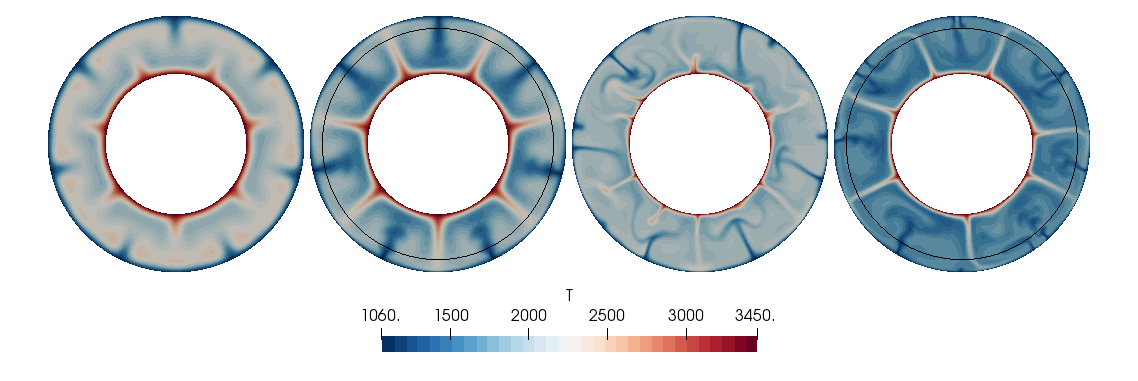
\includegraphics[width=0.9\textwidth]{temps.png}
  \caption{\it Bunge et al.~benchmark. From left to right: temperature field at time $t=5\cdot 10^9$ years obtained with viscosity profiles a, b, c and d.}
  \label{fig:bunge_et_al}
\end{figure}


